\section*{Exercice 1}
\begin{wrapfigure}[10]{r}{5cm}
    \vspace{-1.5cm}
    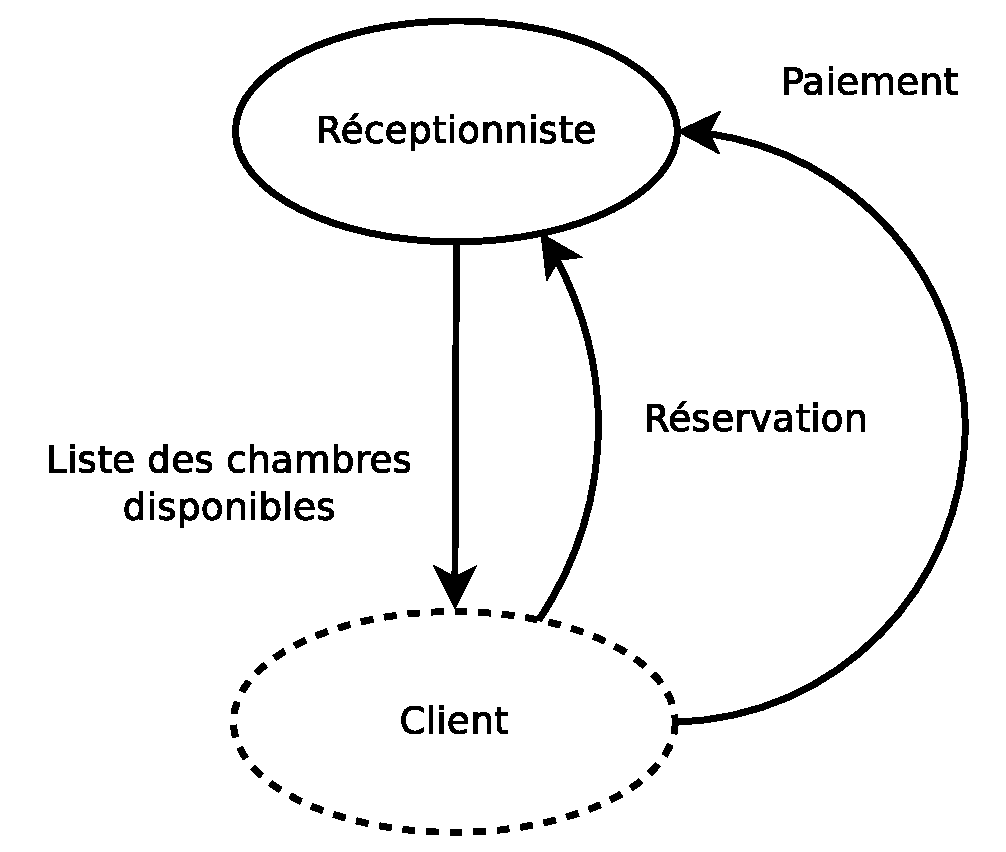
\includegraphics[height=4cm]{mcc.eps} 
    \caption{\label{mcc} Partie du MCC}
\end{wrapfigure}

Un petit hôtel sur la côte souhaite revoir la gestion informatique de ses chambres. Une première partie du MCC a été réalisée sur la Figure~\ref{mcc}. Donnez le MCD correspondant.

\section*{Exercice 2}

L'hôtel souhaite maintenant aller plus loin et réaliser la modélisation complète de son système d'information. Une première étude a mis en évidence les besoins suivants : \\
\begin{itemize}
    \item Le réceptionniste doit pouvoir consulter la description et la disponibilité des chambres pour informer le client.
    \item Le réceptionniste doit pouvoir enregistrer la réservation d'une chambre, et l'annulation de cette réservation pour informer le gérant.
    \item Le réceptionniste doit pouvoir enregistrer le paiement des chambres par les clients.
    \item Le gérant doit pouvoir consulter le taux d'occupation annuel d'une chambre.
    \item On ne veut pas qu'un client puisse réserver plusieurs chambres sur une même période.
    \item Une chambre coûte le même prix toute l'année.
\end{itemize}

\subsubsection*{documents jugés utiles}
\begin{itemize}
    \item Fiche de réservation (nom du client, courriel du client, dates de réservation)
    \item Facture (nom du client, montant, date de paiement)
    \item Fiche descriptive pour chaque chambre (numéro, prix, vue sur la mer)\\
\end{itemize}

Modélisez ce système d'information selon la méthode vue en cours. \textbf{Attention} : le MCC étudié à l'Exercice 1 n'est qu'une partie du MCC qu'il faut modéliser ici.
